\status{started}
\chapter{muEDM entrance detector}
\label{ch:muEDM:entrance}
\begin{refsection}

{\itshape
In the previous chapter, the muEDM experiment was introduced and the current status was described.
In this, we will describe the simulations and beamtimes connected to the entrance detector of the experiment. 
We will start with the \gf simulations of thin and thick scintillators, moving then to the entrance detector and the `telescope' used in the beamtime of 2022.
We will then move through the beamtimes.
}

\status{started}
\section{Short intro to scintillators}
\label{sec:muEDM:scintillators}
    A \textit{scintillator} is any material that emits light (visible or ultraviolet) when exposed to ionizing radiation, like high-energy photons or charged particles.
    The main distinction is between organic and inorganic scintillators:
    \begin{outline}
        \1 Organic scintillators are typically composed of carbon, hydrogen, and other organic (carbon-based) compounds. These materials often include fluorescent dyes or organic molecules that emit light when excited by ionizing radiation.
        They are often used for neutron detection and can also be used for other types of radiation, such as alpha and beta particles. They are versatile and find applications in various fields, including nuclear and particle physics
        \1 Inorganic scintillators are composed of inorganic materials that do not primarily contain carbon-hydrogen (C-H) bonds. These materials can include compounds like sodium iodide (\ce{NaI(Tl)}), cesium iodide (\ce{CsI(Tl)}), bismuth germanate (\ce{Bi4Ge3O12} often "BGO"), and lanthanum halides (\ce{LaBr3} and \ce{LaCl3}).
        These are commonly used in applications requiring high energy resolution and efficiency, like in gamma-ray spectroscopy, high-energy physics experiments, or medical imaging.
    \end{outline}
    Organic scintillators typically have relatively fast response times and are less expensive, while inorganic scintillators tend to have better energy resolution.
    Organic scintillators dived in: liquid, crystaline and plastic.
    We will discuss plastic scintillators while an example of a liquid scintillator, based on Xenon, will be presented when describing the MEG II apparatus (see Ch.\ref{ch:MEG}).

    \status{started}
    \subsection{Plastic scintillators}
        Plastic scintillators are by far the most widely used and their densities range from $1.03$ to $\SI{1.2}{g\per cm^3}$, with a light yield of $1\divisionsymbol\SI{100}{\upgamma/eV}$ of energy deposit \cite{PDG}.
        The number of photons emitted is not linear with the energy deposit: in very dense ionization the light yield is lower than expected.
        This effect is described with the Birks's formula (Eq.~\ref{eq:Birk}) for the luminescence $\mathcal{L}$.

        \begin{equation}
            \dv{\mathcal{L}}{x} = \mathcal{L}_0 \frac{\dv{E}{x}}{1 + k \dv{E}{x}}
            \label{eq:Birk}
        \end{equation}

        Where $\dv{\mathcal{L}}{x}$ is the Light output, $\dv{E}{x}$ the energy loss per unit length by ionizing radiation and $k$ Birks' constant (also known as the stopping power ratio).

        Plastic scintillators are widely used in particle detectors due to their high light yield and fast response time, enabling sub-nanosecond timing resolution. They offer the advantage of pulse shape discrimination, allowing for particle identification based on emitted light during the decay "tail," particularly sensitive to proton recoils from neutrons due to their hydrogen content.

        These scintillators are popular due to their ease of fabrication into various shapes and cost-effectiveness. Scintillating fibers made from plastic scintillators are commonly used in tracking and calorimetry applications.

        \status{started}
        \subsection{Scintillation process}
        Charged particles passing through matter create excited molecules, some of which release about 3\% of their energy as optical photons through a process known as scintillation. This phenomenon is prominent in organic substances containing aromatic rings like polystyrene (PS) and polyvinyltoluene (PVT), as well as in liquids such as toluene, xylene, and pseudocumene.

        In fluorescence, molecules are initially excited by absorbing a photon and then deexcite by emitting a longer wavelength photon. To shift scintillation light to a more convenient wavelength, fluorescent materials, or "fluors," are used as "waveshifters." However, complex molecules in fluorescence can exhibit self-absorption, which shortens the attenuation length. The greater the Stokes' shift (the difference between absorption and emission wavelengths), the less self-absorption occurs, making a larger Stokes' shift desirable for fluors.

        In high-energy physics, plastic scintillators are typically composed of selected fluors dissolved in a plastic base containing aromatic rings. Most plastic scintillators use either PVT or PS as their base, with PVT-based scintillators being up to 50\% brighter. Adding a "primary" fluor in high concentration (1\% by weight) into the base helps improve the attenuation length, as it efficiently re-radiates absorbed energy at wavelengths where the base is more transparent.

        The primary fluor also plays a crucial role in shortening the scintillator's decay time, increasing the total light yield. The strong coupling between the base and fluor, known as Foerster resonance energy transfer, occurs at short distances, enhancing the speed and light yield of plastic scintillators.

        In some cases, when the selected fluor doesn't meet all requirements, a "secondary" fluor may be added in fractional percent levels, and occasionally even a third.

        External wavelength shifters are employed to aid light collection in complex geometries. They consist of a lightpipe with a wave-shifting fluor dissolved in a non-scintillating base. Typically, an acrylic base is used for its optical qualities, along with a single fluor to shift the emitted light to the blue-green range. These shifters also contain additives to absorb ultraviolet light and reduce sensitivity to Cherenkov radiation.

        For specialized applications, scintillators with increased radiation resistance or unique properties like neutron/gamma discrimination can be created by significantly increasing fluor concentrations.
        
        \status{started}
        \subsection{Scintillating Fibers}
        This is also a good moment to introduce The concept of \textit{scintillating fibres}.
        We will not use them in this chapter but will be key in Ch.~\ref{ch:muEDM:tracker}, dedicated to the $\Ae$ tracking.
        
        The use of clad optical fibers containing scintillators and wavelength shifters (WLS) has proven highly beneficial. Scintillating fiber (SCIFI) calorimeters, first demonstrated in [45], have become mainstream due to their speed, density, radiation resistance, and impressive resolution akin to lead glass. SCIFI trackers can handle high rates and radiation but require sensitive photodetectors due to low photon yield at the fiber's end. 

        Control over the sensitive region of scintillating fibers can be achieved by splicing them onto clear, non-scintillating fibers.

        Typically, these fibers have a core of polystyrene-based scintillator or WLS (refractive index n = 1.59), surrounded by a cladding of PMMA (n = 1.49), sometimes with an additional fluorinated PMMA cladding (n = 1.42) for enhanced light capture, resulting in a diameter of 0.5 to 1 mm. The capture fraction, representing the proportion of generated light transported down the optical fiber, is around 6\% for single-clad fibers and 10\% for double-clad fibers. A minimum-ionizing particle traversing a 1 mm diameter fiber perpendicularly generates fewer than 2000 photons, with approximately 200 captured. In a large collider tracker, attenuation may eliminate up to 95\% of these photons.

        The attenuation length, the distance over which the signal diminishes to 1/e of its original value, is influenced by factors such as re-absorption of emitted photons, polymer base crystallinity, photodetector sensitivity, and internal surface quality. High-quality fibers can achieve attenuation lengths of several meters.
        
\status{started}
\section{\gf simulations}
    \label{sec:muEDM:entrance:sim}
    \status{review}
    \subsection{\gf}
        \gf (GEometry ANd Tracking) is a powerful open-source simulation toolkit used in various scientific fields, primarily for studying the interactions of particles with matter, and is widely employed in particle, nuclear, and medical physics. 
        At its core, \gf works by representing the physical world as a set of geometric shapes and materials. 
        After defining the properties of particles, their energy, and the materials they interact with, \gf simulates their behavior. 
        This toolkit utilizes a range of physics models and algorithms to accurately model particle interactions, including electromagnetic, hadronic, and optical processes. It can simulate particles of various energies, from subatomic to cosmic ray levels.
        The simulation is \textit{step} based: at every interaction, the physical properties of the particle are updated and, if needed, secondary particles are generated. 
        Steps are forced to end when crossing the boundary between two materials/volumes to ensure proper care is taken in the transition. 
        This is of particular importance for optical simulations, such as the propagation of OpticalPhotons produced by scintillation.

    \status{started}
    \subsection{Entrance system}
        To study the feasibility of the entrance thin scintillator, a \gf simulation was developed.
        The first step, after achieving a running simulation of scintillation, was to study the range of muons of the interesting momenta, as well as the energy deposit. 
        These first results are shown in Fig.~\ref{fig:muEDM:entrance:edep}.
        Here we can see the energy deposit for $\Ae$ and $\Am$ in scintillators of different thicknesses, reflecting the well-known Bethe-Bloch plot shown in Fig.~\ref{fig:muEDM:entrance:BetheBloch}. 
        Interesting features are:
        \begin{outline}
            \1 The energy deposit is linear with the thickness for the $\Ae$
            \1 The linearity is lost for the $\Am$. First, we have an exponential trend and then a plateau, when $E_{dep}\approx E_k$ and the $\Am$ is stopped
            \1 The shape of the deposit slowly changes from Landau to Gaussian
        \end{outline}
        In Fig.~\ref{fig:muEDM:entrance:edep:log} we recover the linear (and then exponential) trend when sampling the energy deposit for $\Am$ for lower thicknesses at both \SI{28}{MeV/c} and \SI{128}{MeV/c}.


        \begin{figure}
            \centering
            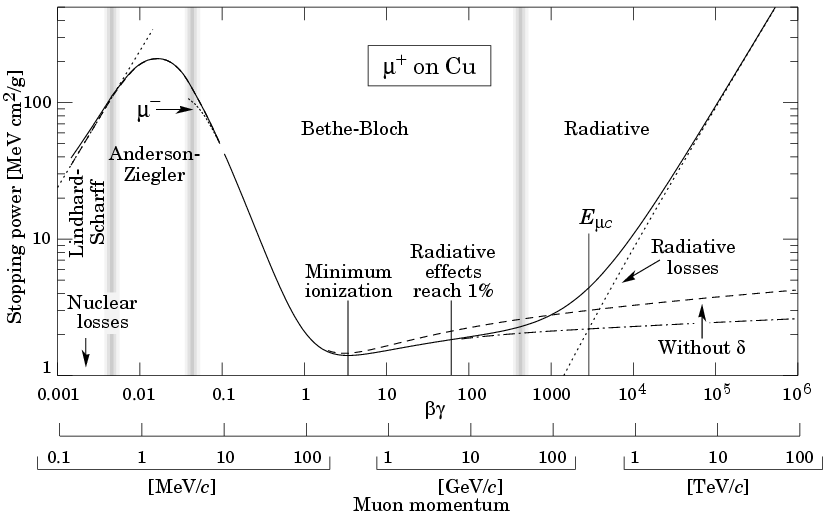
\includegraphics[width=0.9\textwidth]{Figures/muEDM/Entrance/BetheBloch.png}\\
            \caption{This figure illustrates the Bethe-Bloch formula \cite{PDG}, a vital tool in particle physics, depicting how charged particles lose energy when traversing through matter.}
            \label{fig:muEDM:entrance:BetheBloch}
        \end{figure}
        
        \begin{figure}   
            \centering
            \subfloat[A \SI{28}{MeV\per c} $\Ae$ has $E_k \approx \SI{27.5}{MeV}$.]{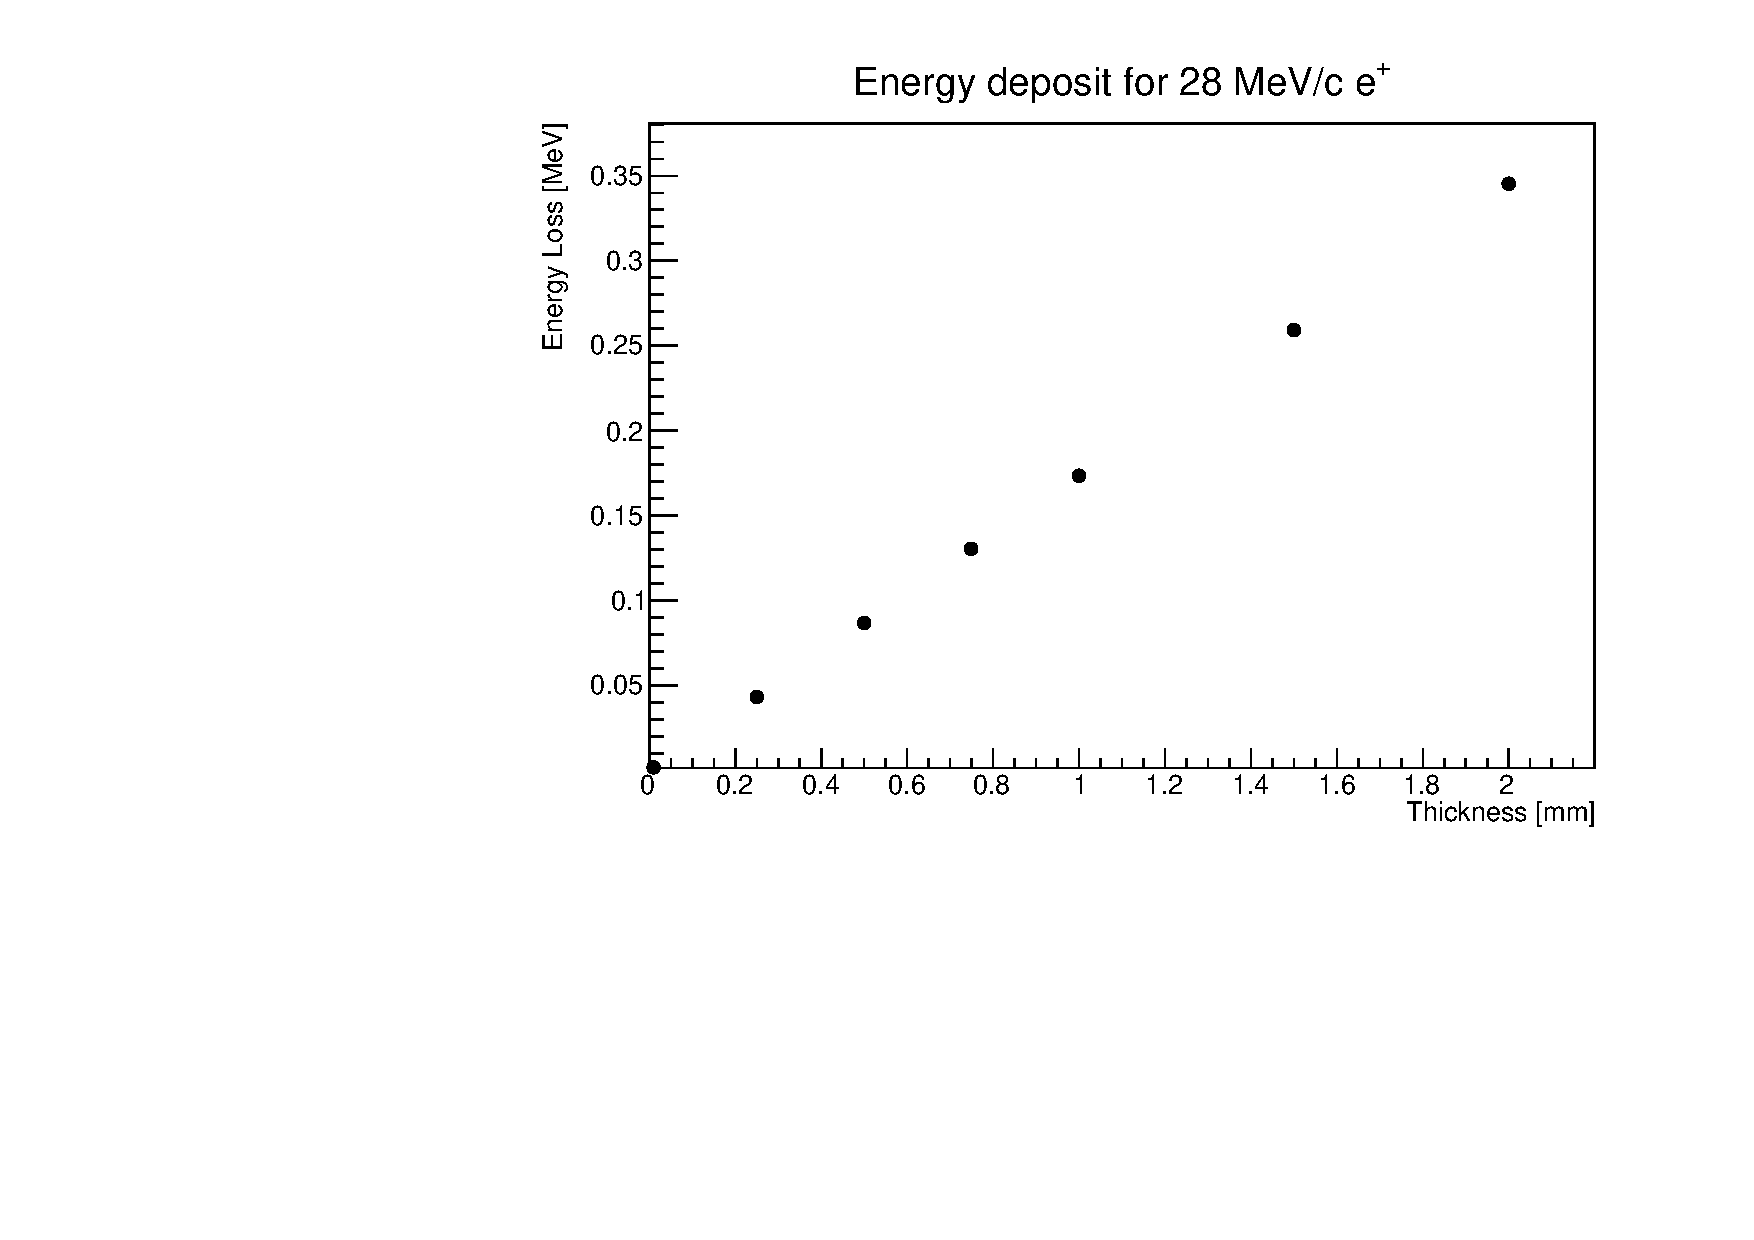
\includegraphics[height=5.5cm, keepaspectratio]{Figures/muEDM/Entrance/e_28_thick.pdf}\label{fig:muEDM:entrance:edep:e28}}
            \hfill
            \subfloat[AAA]{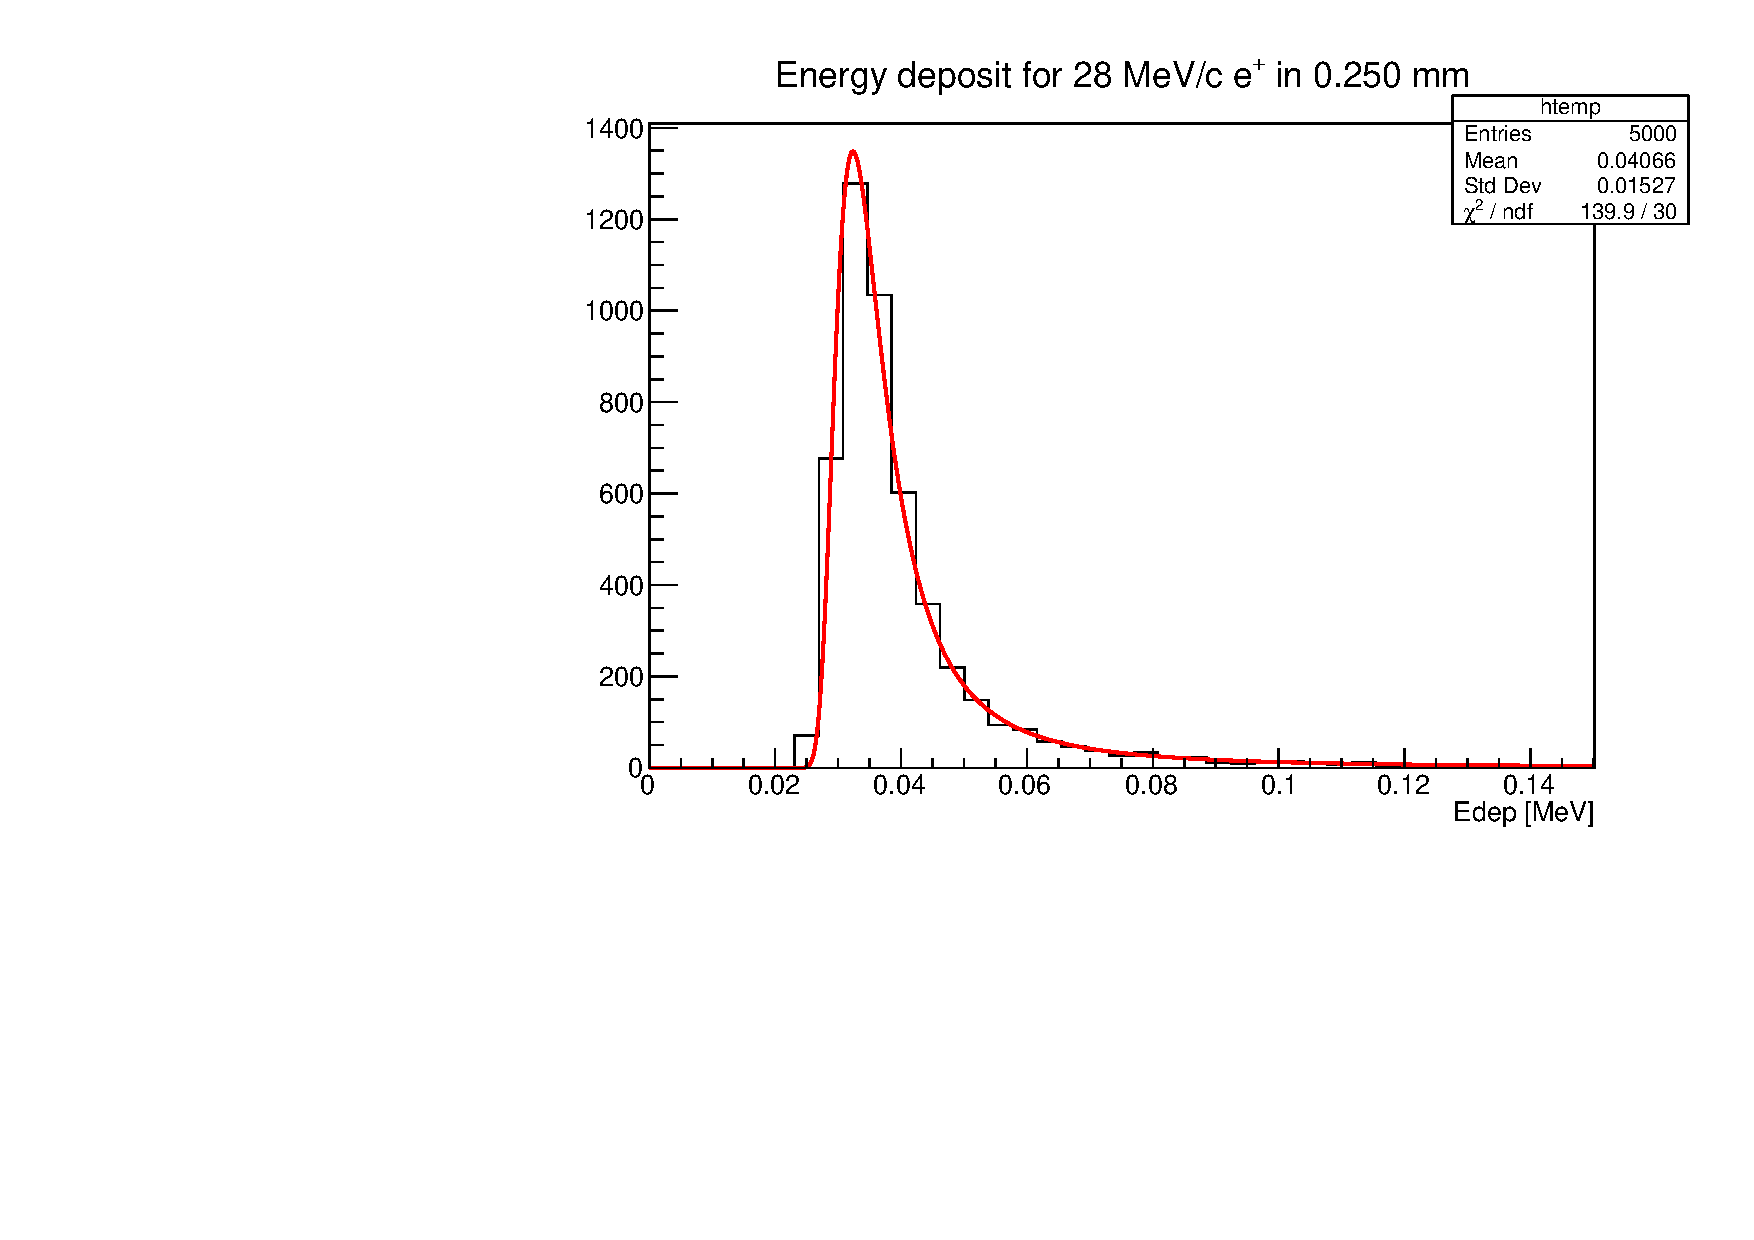
\includegraphics[height=5.5cm, keepaspectratio]{Figures/muEDM/Entrance/e_28_Edep_0.250.pdf}\label{fig:muEDM:entrance:edep:e28_0.25}}\\
            \subfloat[A \SI{28}{MeV\per c} $\Am$ has $E_k \approx \SI{3.6}{MeV}$.]{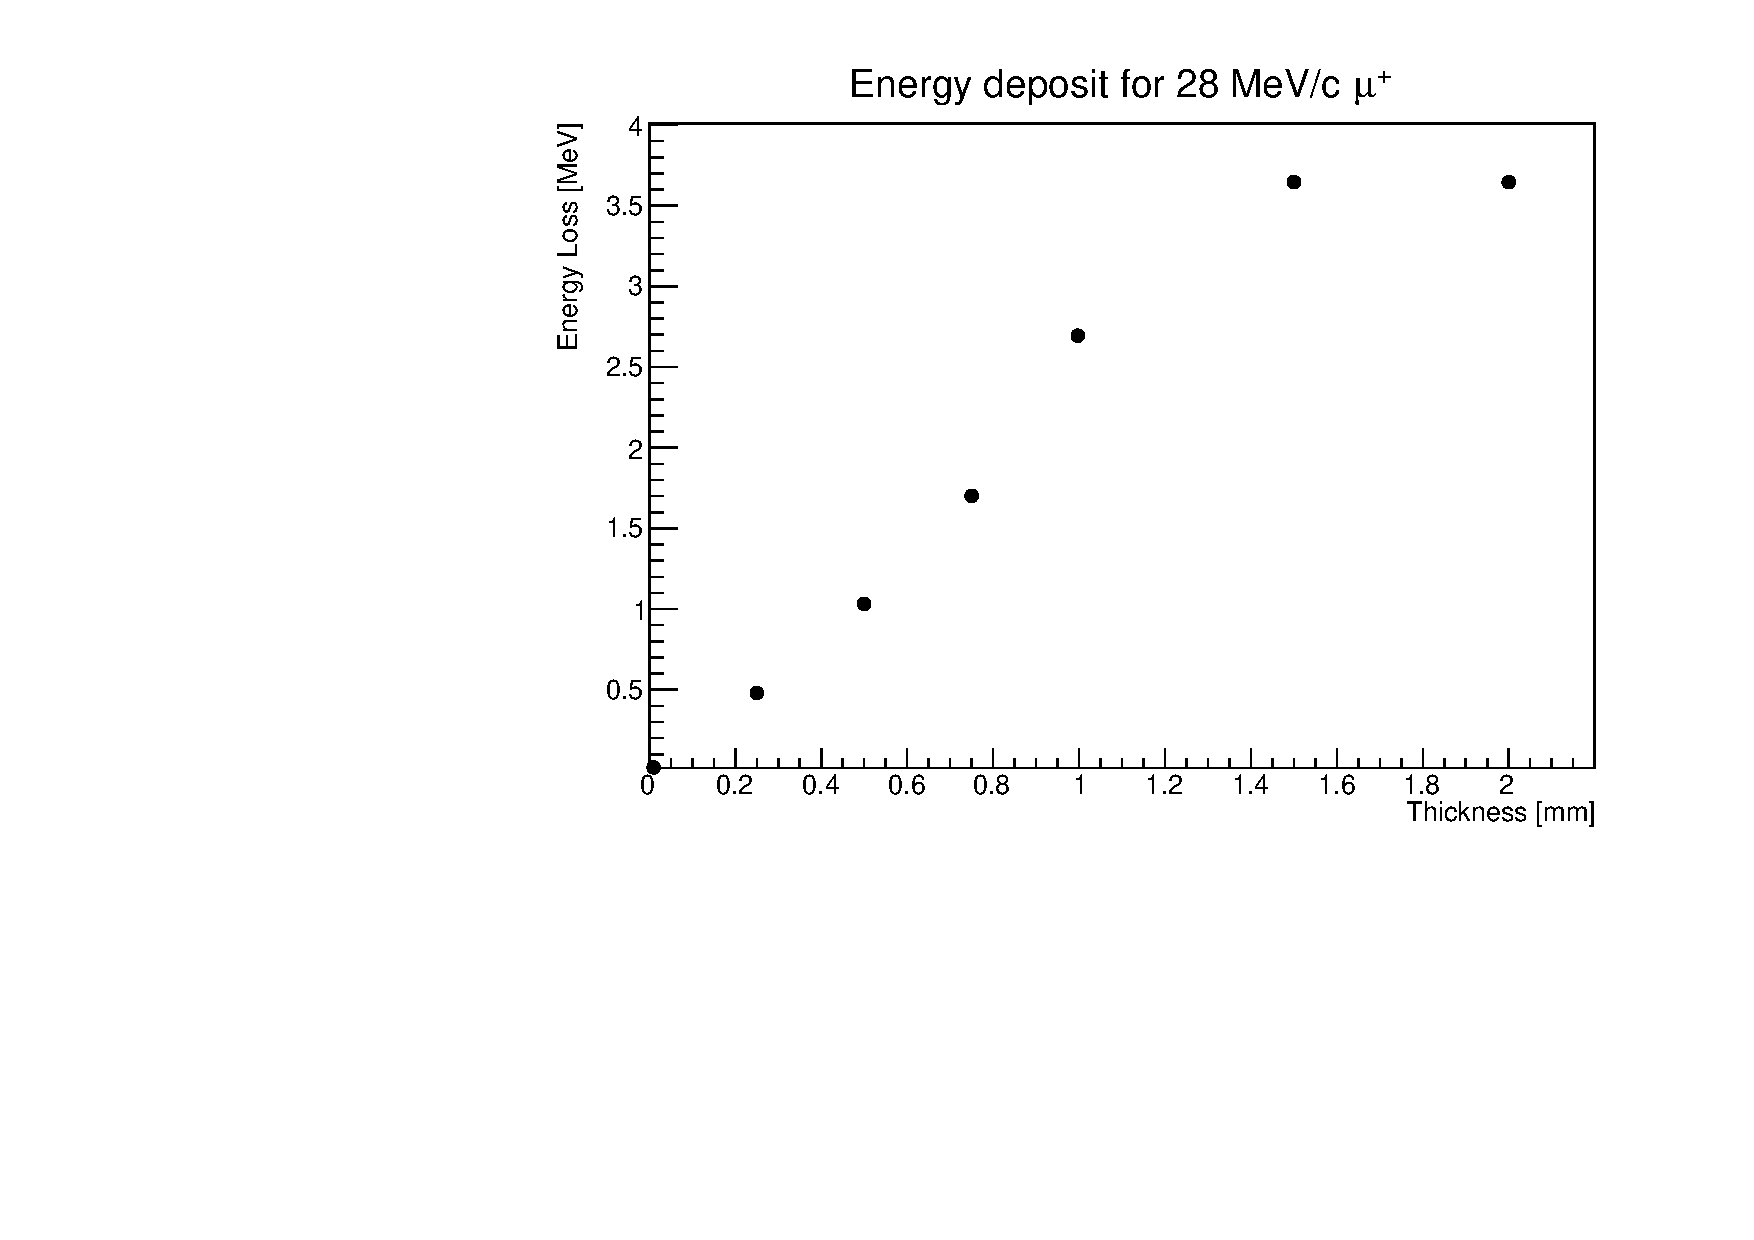
\includegraphics[height=5.5cm, keepaspectratio]{Figures/muEDM/Entrance/mu_28_thick.pdf}\label{fig:muEDM:entrance:edep:mu28}}
            \hfill
            \subfloat[AAA]{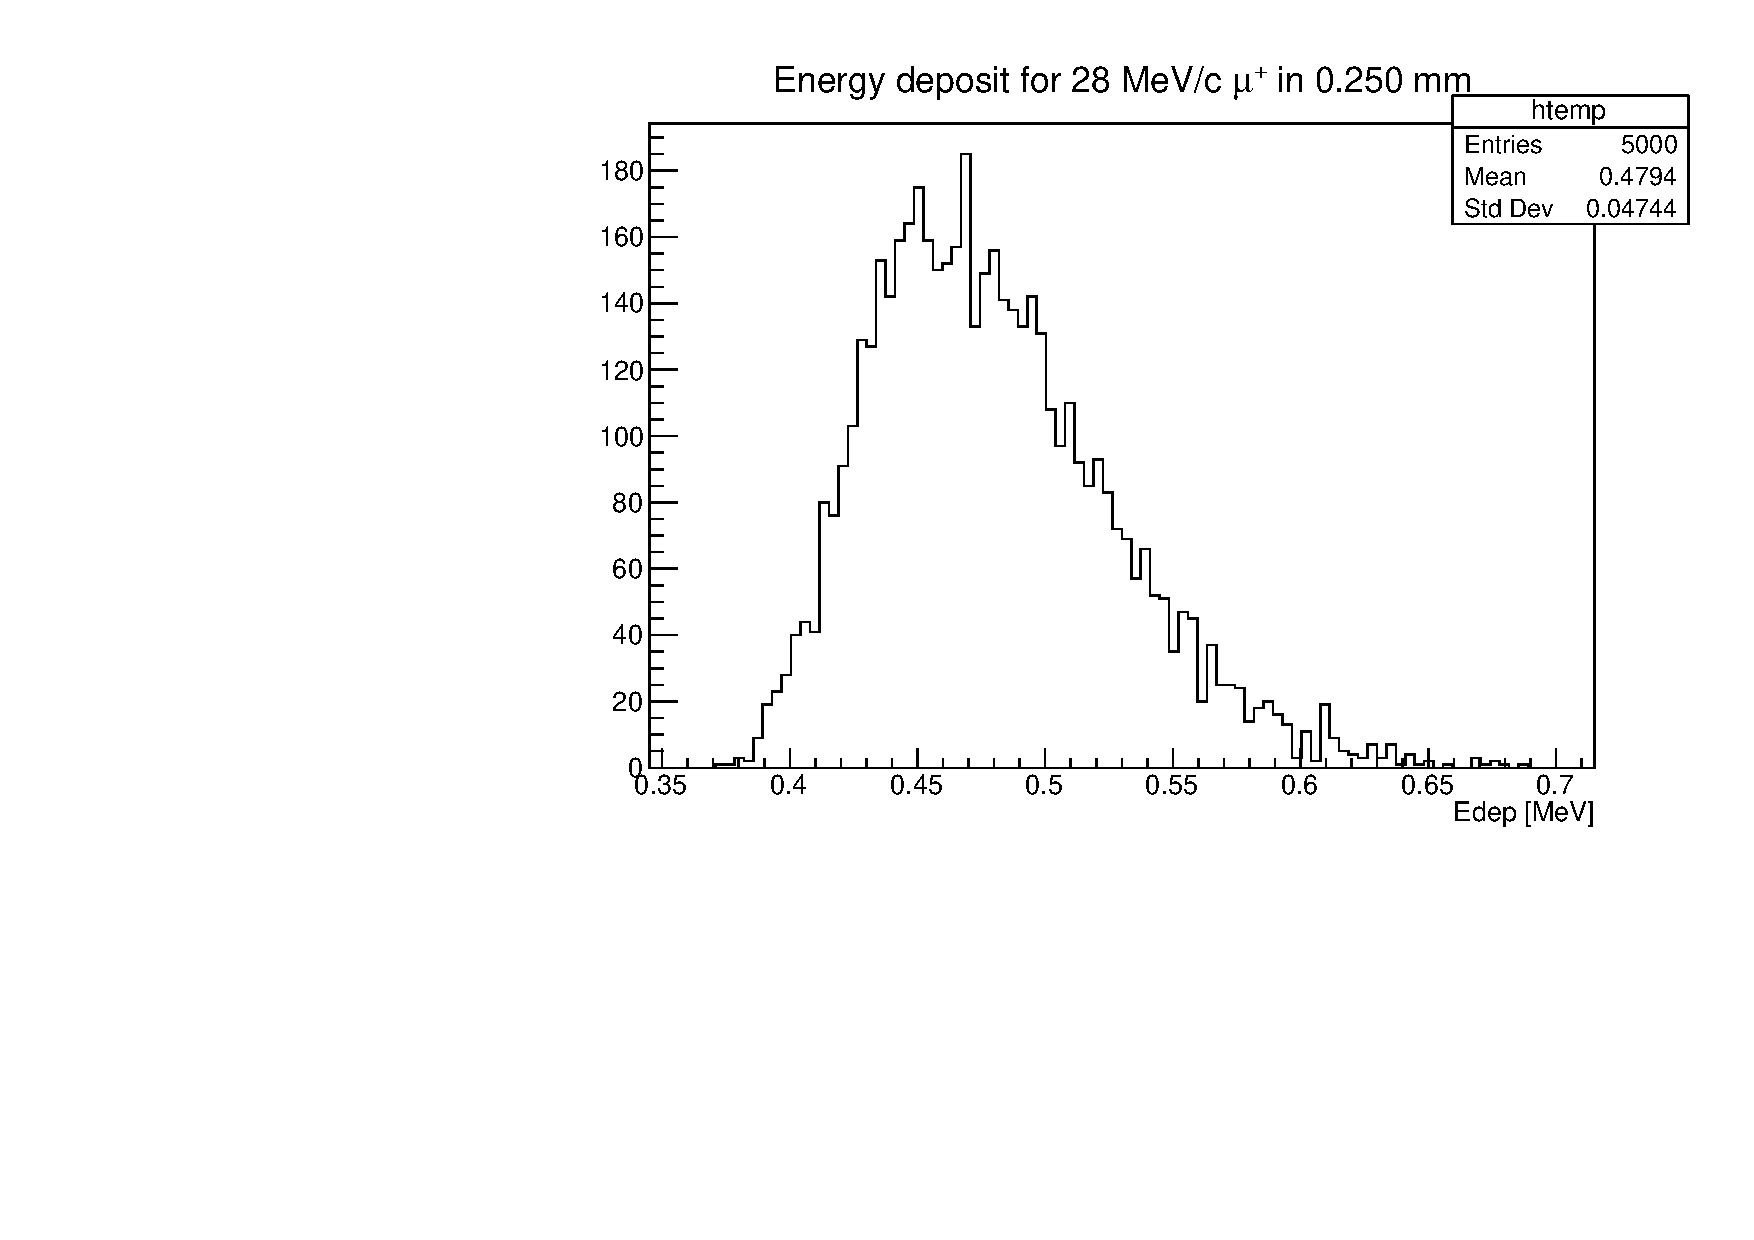
\includegraphics[height=5.5cm, keepaspectratio]{Figures/muEDM/Entrance/mu_28_Edep_0.250.pdf}\label{fig:muEDM:entrance:edep:mu28_0.25}}
            \caption{Curve for the average energy deposit in a \bc{400} scintillator for $\Am$ (\ref{fig:muEDM:entrance:edep:e28}) and $\Ae$ (\ref{fig:muEDM:entrance:edep:mu28}) at \SI{28}{MeV\per c}. Clearly visible is the linearity of the energy loss for the $\Ae$ with thickness. This linearity is lost for the $\Am$: first, we see an exponential trend and then a plateau when $E_{dep}\approx E_k$ and the $\Am$ is stopped. The distribution of the energy deposit slowly transitions from a Landau to a Gaussian: (\ref{fig:muEDM:entrance:edep:e28_0.25}) is an example of the first type; (\ref{fig:muEDM:entrance:edep:e28_0.25}) is an example of the transition.}
            \label{fig:muEDM:entrance:edep}
        \end{figure}
        
        \begin{figure}   
            \centering
            \subfloat[A \SI{28}{MeV\per c} $\Am$ has $E_k \approx \SI{3.6}{MeV}$.]{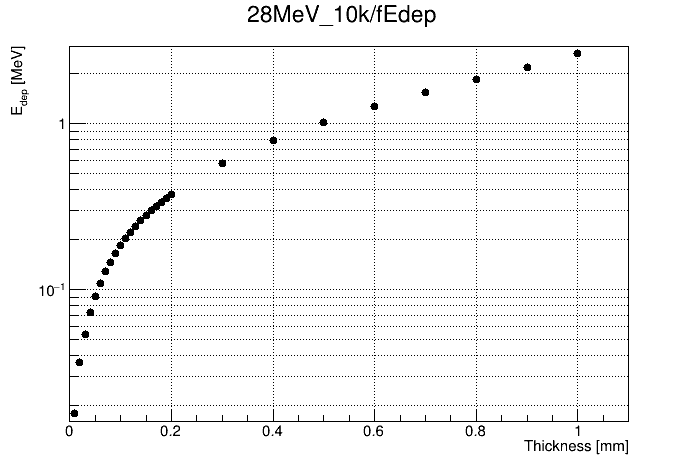
\includegraphics[height=5.5cm, keepaspectratio]{Figures/muEDM/Entrance/28mu_edep.png}\label{fig:muEDM:entrance:edep:log:28}}
            \hfill
            \subfloat[A \SI{128}{MeV\per c} $\Am$ has $E_k \approx \SI{60.3}{MeV}$.]{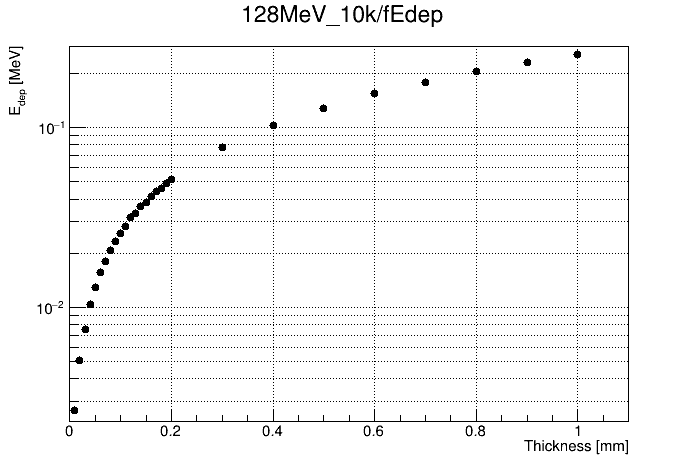
\includegraphics[height=5.5cm, keepaspectratio]{Figures/muEDM/Entrance/128mu_edep.png}\label{fig:muEDM:entrance:edep:log:128}}
            \caption{Detail on the lower section of the curve for the average energy deposit in a \bc{400} scintillator for $\Am$ at \SI{28}{MeV\per c} and \SI{128}{MeV\per c}.}
            \label{fig:muEDM:entrance:edep:log}
        \end{figure}

        \subsubsection{Multiple scattering}
            An important sanity check was also to study the multiple scattering in the scintillator. 
            More details on the functional description and the \gf implementation of the multiple scattering will follow, in \ref{sec:muEDM:tim}.
            This was done with a fit to the Highland formula (Eq.~\ref{eq:highland}) the average value of the scattering angle as a function of the thickness. 
            These fits are shown in Fig.~\ref{fig:muEDM:entrance:ms} and the results, $X_{0, 28MeV} = \SI{54.36(17)}{gm/cm^2}$ and $X_{0, 128MeV} = \SI{54.30(14)}{gm/cm^2}$, are consistent with the value for \bc{400} of $X_{0}\sim 50$.

        \subsubsection{Thickness and number of photons}
            
        \begin{figure}
            \centering
            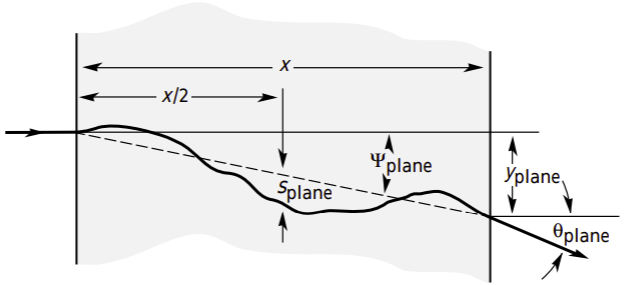
\includegraphics[width=0.6\textwidth]{Figures/muEDM/Entrance/multiple-scattering_pdg.png}\\
            \caption{}
            \label{fig:muEDM:entrance:pdgms}
        \end{figure}

        \begin{figure}   
            \centering
            \subfloat[ASD]{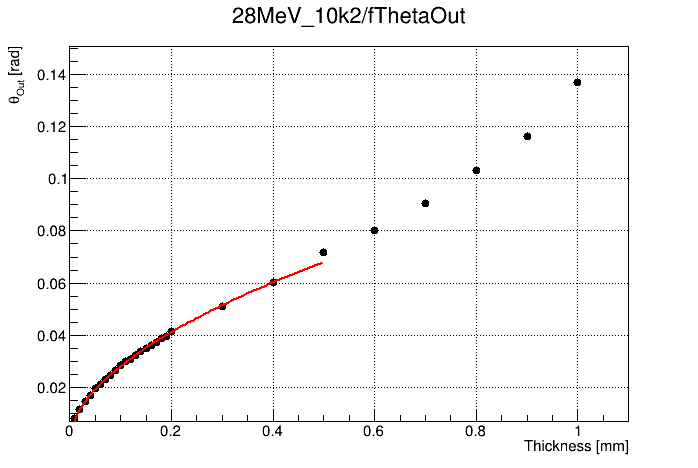
\includegraphics[height=5.5cm, keepaspectratio]{Figures/muEDM/Entrance/28mu_angleout_fit.png}\label{fig:muEDM:entrance:ms:28}}
            \hfill
            \subfloat[ASD]{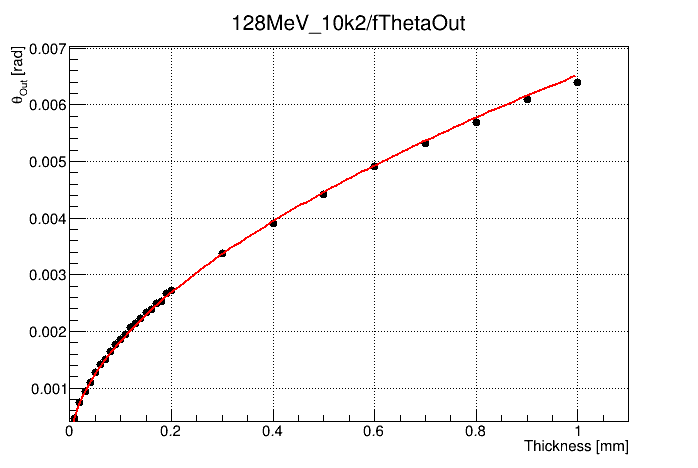
\includegraphics[height=5.5cm, keepaspectratio]{Figures/muEDM/Entrance/128mu_angleout_fit.png}\label{fig:muEDM:entrance:ms:128}}
            \caption{Average scattering angle in different thicknesses of \bc{400} scintillator for $\Am$ at \SI{28}{MeV\per c} and \SI{128}{MeV\per c}. From these plots was found $X_0 = \SI{54.33(12)}{g/cm^2}$.}
            \label{fig:muEDM:entrance:ms}
        \end{figure}
        
        \subsubsection{Detection of photons}
            Not all photons produced will be detected.
            This is affected by the position, number, size, and PDE\footnote{Photon detection efficiency describes the effectiveness of a photon detector in registering incoming photons. It quantifies the probability that a photon incident on the detector will be detected and converted into an electrical signal} of the SiPMs. 
            To simulate the SiPM readout we can use a silicon volume coupled to the scintillator via an additional volume of optical grease\footnote{Also known as optical coupling grease or index-matching grease, is a specialized type of grease used in optics and photonics applications. It is designed to improve the optical coupling between two optical components, such as lenses, prisms, or optical fibers.}.
            Multiple readouts would allow us to lower the threshold and improve the dark noise rejection. Calling the sides $s_i$, the options could be $(s_1\land s_3)\lor(s_2\land s_4)$, $(s_1\land s_3)\land(s_2\land s_4)$, or simply $(s_1\land s_3)$.
            We studied these different readouts schemes in the beamtime of Dec. 2023 (see Sec.~\ref{muEDM:beamtime2023}) 

        \begin{figure}
            \centering
            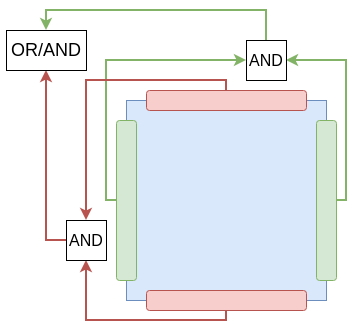
\includegraphics[height = 5cm]{Figures/muEDM/Entrance/gate_multireadout.png}
            \caption{Multiple readouts of a thin scintillator to lower the threshold and improve the dark noise rejection. Possible schemes are $(s_1\land s_3)\lor(s_2\land s_4)$, $(s_1\land s_3)\land(s_2\land s_4)$, or simply $(s_1\land s_3)$.}
            \label{fig:muEDM:entrance:gate:readout}
        \end{figure}
        
    \subsection{Telescope and entrance detector}
        \begin{figure}   
            \centering
            \subfloat[ASD]{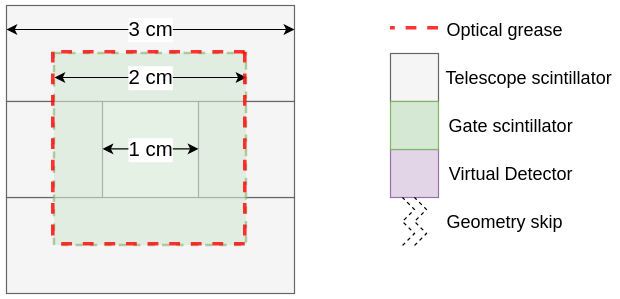
\includegraphics[height=4.5cm, keepaspectratio]{Figures/muEDM/Entrance/gate_geometry.png}\label{fig:muEDM:entrance:ms:28}}
            \hfill
            \subfloat[ASD]{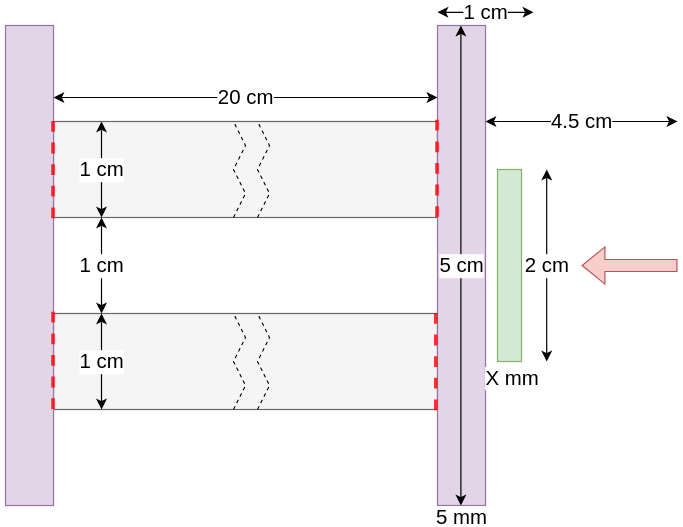
\includegraphics[height=5.5cm, keepaspectratio]{Figures/muEDM/Entrance/entrance_geometry.png}\label{fig:muEDM:entrance:ms:128}}
            \caption{}
            \label{fig:muEDM:entrance:sketches}
        \end{figure}
        
\status{started}
\section{Beamtime 2021}
\label{sec:muEDM:tim}
    This was the first muEDM beamtime I participated in. 
    I took an active part in the setup and measurement and I followed the analysis of the data collected. 
    This section relies on the Master Thesis of Tim Hume, part of the muEDM collaboration.
    This beamtime was designed to study the positron multiple scattering in different thin foils of the material expected to be viable solutions for the different parts of the experiment.
    On top of the material details, the aim was also to validate the scattering model used in the \gf simulations for further reference.
    The setup was quite simple: a telescope of five silicon pixel sensors,  three upstream and two downstream.

    \status{started}
    \subsection{Description of the multiple scattering}
        \paragraph{Highland}
        The Highland formula for multiple scattering is a parameterization for the width of the multiple scattering distribution.
        For a particle of charge $z$, momentum $p$ traversing a thickness of $x$ of a material with radiation length $X_0$, the RMS of the gaussian distribution is estimated as:
        \begin{equation}
        \label{eq:highland}
        \theta_0 = \frac{\SI{13.6}{MeV}}{\beta p c} z \sqrt{\frac{x}{X_0}} \left(1 + 0.038 \ln( \frac{x z^2}{X_0 \beta^2}) \right)
        \end{equation}
        Often, in the context of high particle physics, the projection on the directions orthogonal to the momentum are considered:
        \begin{equation}
        P(\theta_{x,y}) = \frac{1}{{\theta_0 \sqrt{2\pi}}} \exp\left(-\frac{\theta_{x,y}^2}{2\theta_0^2}\right)
        \end{equation}

        \paragraph{\gf}
        The default parameterization of the multiple scattering in \gf is the Urb\'{a}n. This is based on a different description of the process, required because when evaluating the processes at each step of the simulation, meaning \textit{within} the volume.
        This model describes the angular distribution of multiple scattering and samples it every interaction.
        The probability density of the angular distribution is usually indicated with $g(u)$ where $u = \cos \theta$ and the form is the following:
        \begin{equation}
            g(u) = \alpha +
            \begin{cases}
                \beta \exp(\gamma u) &\text{for } u_0 \le u \le 1 \\
                \delta (1-u)^\epsilon &\text{for } -1 \le u < u_0
            \end{cases}
        \end{equation}
        The parameter $u_0$ is the one used to transition between the central Gaussian-like distribution and the Rutherford-like tails at larger angles.\\

        \noindent
        For the Highland formula, the PDG reports an accuracy of $\sim 10\%$ in the range $\num{e-3}<x/X_0<\num{e2}$ \cite{PDG}, meaning it is less reliable for thin targets for which $x/X_0 \sim \mathcal{O}(\num{e-4})$.
        On the other hand, while \gf results have been widely tested against experimental measurements, there is a lack of data to compare in the ranges we are interested in.

    \status{started}
    \subsection{Data taking}
        The idea behind the data taking is quite simple: a study on the multiple scattering can be performed using a beam telescope, such as the one sketched in Fig~\ref{fig:muEDM:beamtime2021:telescope}, in which the two sides of the telescope are used to track the in/out-coming particles. 
        The delicate point is to carefully take into account the scattering of the particles in the telescope itself. 
        It is then needed to collect data without the sample to apply a deconvolution of the telescope response.
        The downstream part of the detector is not symmetrical to the upstream because only five sensors had the necessary performance. This made the tracking task more challenging, leading to wider distributions.
        The beamline used is the $\pi$E1, which provides $\uppi^\pm,\upmu^\pm,e^\pm$ in a momentum range \SI{100}{MeV} to \SI{500}{MeV}.
        Clearly, a good understanding of the beam is key in both data-taking and analysis. 
        An example is the study of the beam changing the degrader's thickness, shown in Fig.~\ref{fig:muEDM:beamtime2021:TOF}.
        For brevity, the description of the electronics and DAQ system will be skipped. 

        \paragraph{Silicon Pixel Sensors}
        The sensors used are the last iteration of the sensors of the \textit{mu3e} experiment, the MuPix10. 
        These are High Voltage Monolithic Active Pixel Sensors (HV-MAPS) with $250\times256$ pixels of dimensions \SI{80}{\micro m}$\times$\SI{80}{\micro m}. 
        The sensor itself is on a PCB used for delivering the required voltages.
        A second, larger, PCB is set below the first and is responsible for reading and transmitting the data to FPGA.
        These sensors have been developed to achieve excellent position and time resolutions (\SI{100}{\micro m} and \SI{20}{ns}) with efficiency of $\varepsilon \approx 0.99$. 
        The thickness of these sensors is \SI{50}{\micro m} but this was the case for just the detector positioned after the samples. 
        The others were \SI{100}{\micro m}, important to be considered during the analysis.
        The whole apparatus is shown in Fig.~\ref{fig:muEDM:beamtime2021:setup:telescope} while a singular MuPix10 is shown in Fig.~\ref{fig:muEDM:beamtime2021:setup:MuPix10}.
        
        \begin{figure}
            \centering
            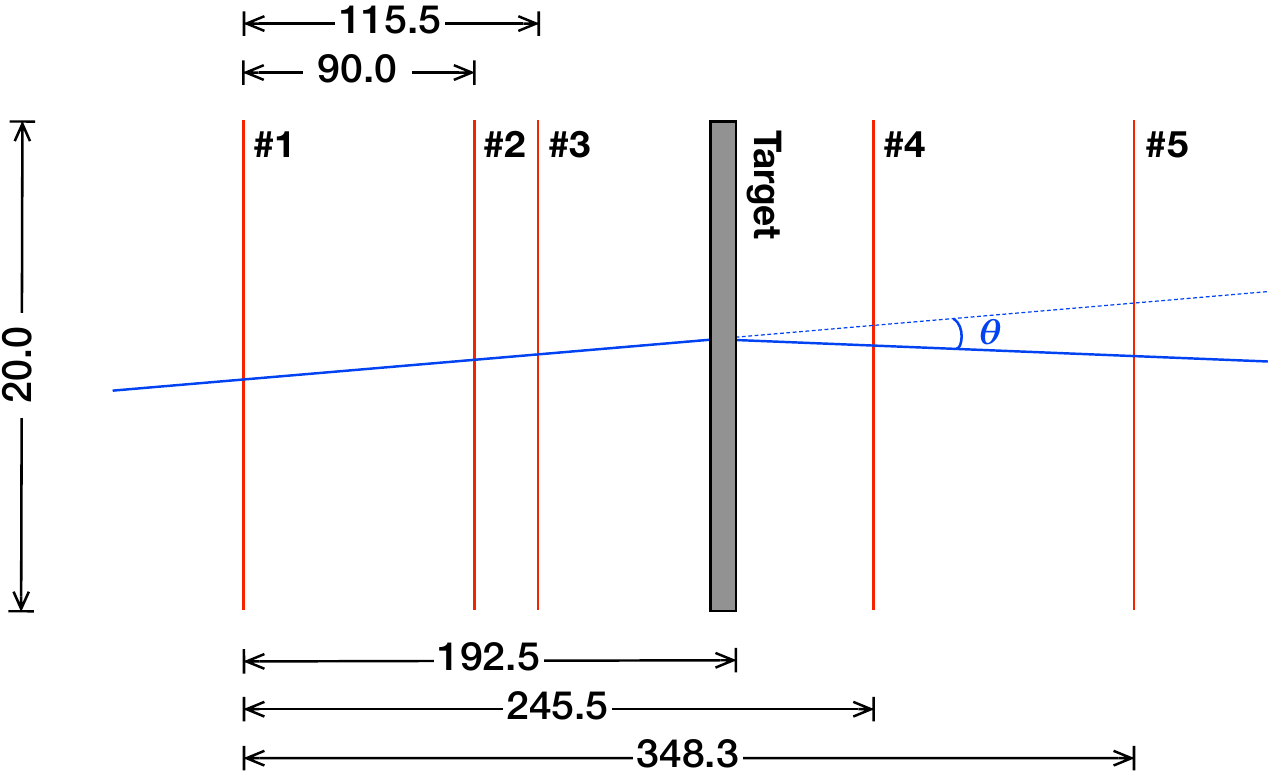
\includegraphics[width=0.6\textwidth]{Figures/muEDM_Dec2021/Positions_Telescope.png}\\
            \caption{Sketch of the telescope of Silicon Pixel Sensors used to study the multiple scattering in different materials.
            The samples are held in the position of the 'target'. 
            In this sketch, the beam is coming from the left side.}
            \label{fig:muEDM:beamtime2021:telescope}
        \end{figure}

        \begin{figure}   
            \centering
            \subfloat[Picture of the setup for the beamtime of 2021. On the right, the scintillator was used as an external trigger, on the left, beam exit window.]{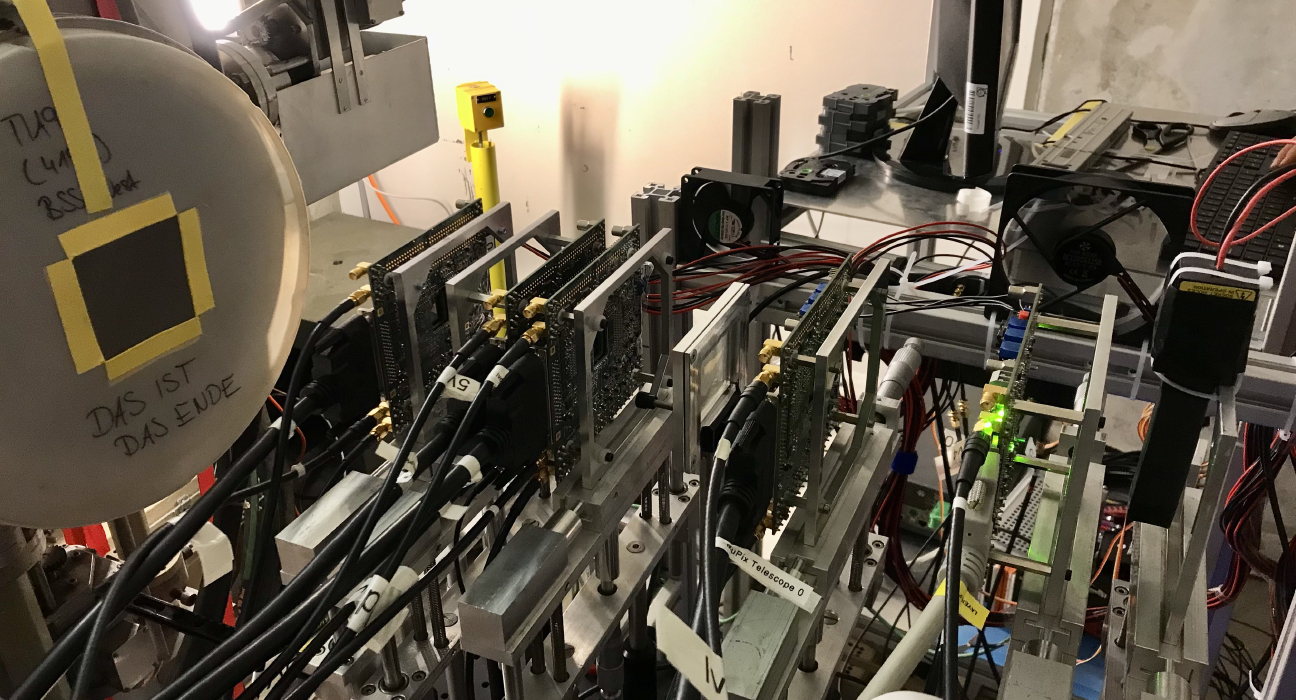
\includegraphics[height=5.5cm, keepaspectratio]{Figures/muEDM_Dec2021/Telescope_Picture.png}\label{fig:muEDM:beamtime2021:setup:telescope}}
            \hfill
            \subfloat[Picture of one of the MuPix10 mounted on the two PCBs.]{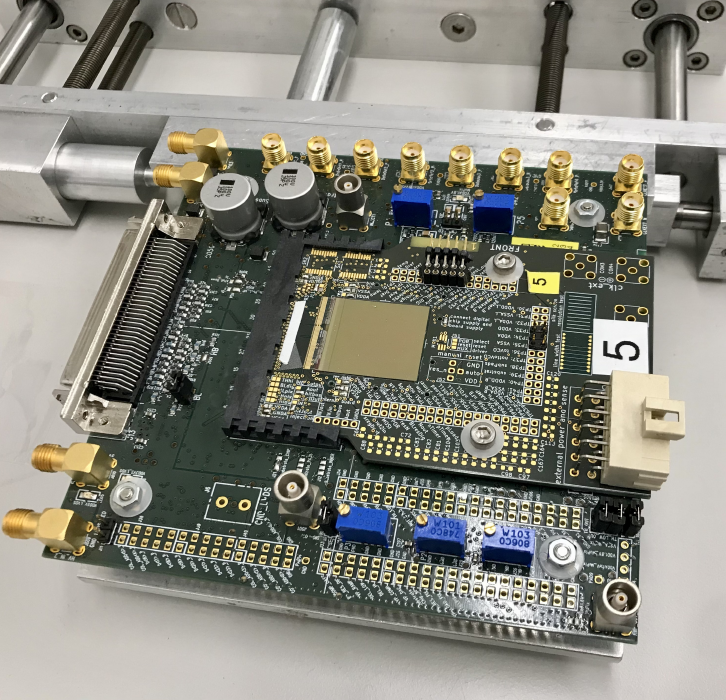
\includegraphics[height=5.5cm, keepaspectratio]{Figures/muEDM_Dec2021/MuPix10_Picture.png}\label{fig:muEDM:beamtime2021:setup:MuPix10}}
            \caption{Picture of the setup and one of the MuPix10 (grey-colored square) mounted on the PCBs.}
            \label{fig:muEDM:beamtime2021:setup}
        \end{figure}

        \begin{figure}
            \centering
            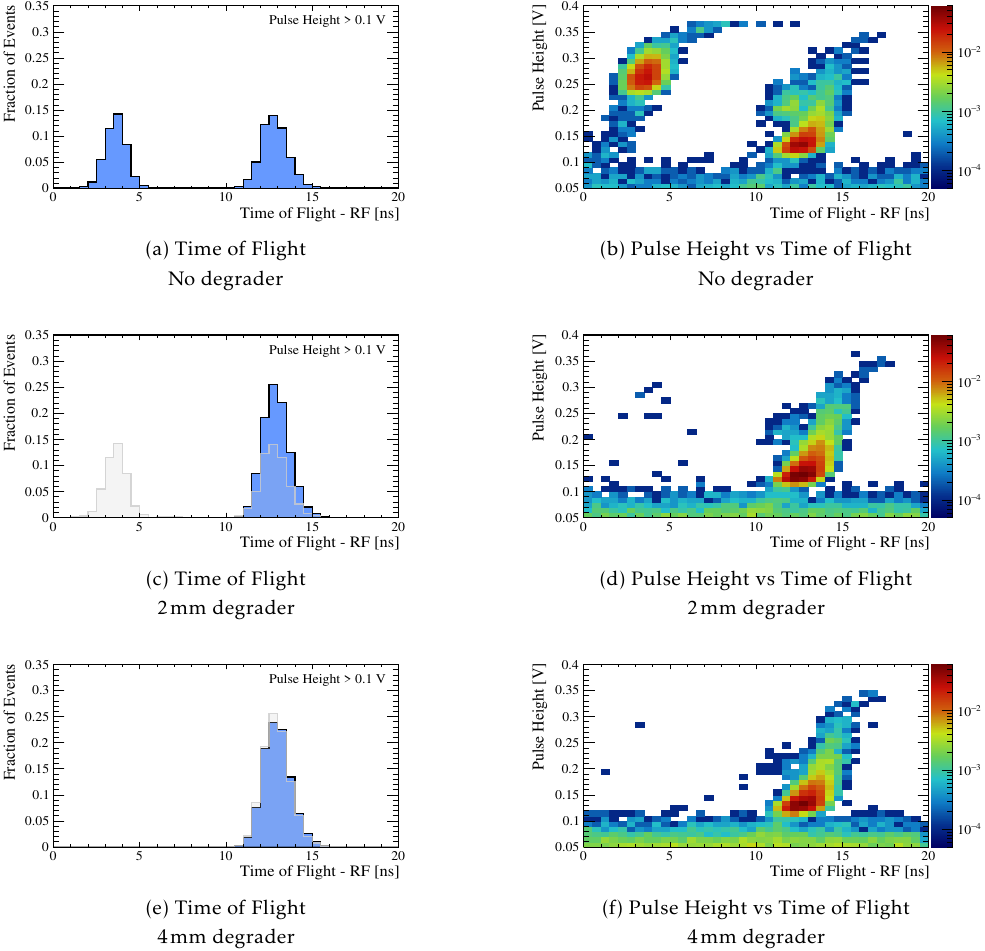
\includegraphics[width=0.9\textwidth]{Figures/muEDM_Dec2021/muEDM_beamtime2021_TOF.png}
            \caption{Timing and the 2D plot for time and pulse height for \SI{120}{MeV/c} particles. The three rows show what happens when inserting degraders of different thicknesses.
            With no degrader, the $\uppi$ peak is visible at lower TOF.
            When increasing the thickness, the contributions of $\uppi$ and $\upmu$ decrease.
            It is important to note that the $e$ and $\upmu$ distribution overlap.
            In gray the distribution of the previous plot to make a comparison.}
            \label{fig:muEDM:beamtime2021:TOF}
        \end{figure}

    \status{started}
    \subsection{Data analysis}
        \paragraph{Track selection}
        Initial angular distributions obtained were broad due to noise in downstream sensors, making it difficult to distinguish noise from true hits. 
        To address this, a filtering process was developed to select the track candidate with the least spatial separation between the intersections of upstream and downstream tracks on the plane of the sample.
        The expected angular distribution for particles passing through a material at normal incidence should be spatially symmetric and independent of chosen projection axes. 
        Any deviation from this symmetry could indicate experimental, data processing, or analysis errors. 
        To mitigate the effects the idea was to combine distributions from multiple axes.
        In the initial distributions, the broad background can be attributed to false tracks generated by noise, poor fits, and some contribution of events with large angles of scattering in the telescope itself. 
        This background was suppressed by enforcing a distance of \SI{1}{mm} between the points at which the upstream and downstream tracks intersect the plane of the sample.        
        Distributions before and after applying this filter are shown in black and red in Fig.~\ref{fig:muEDM:beamtime2021:distributions}
        This distribution was then corrected for the geometric acceptance of the telescope.
        \begin{figure}
            \centering
            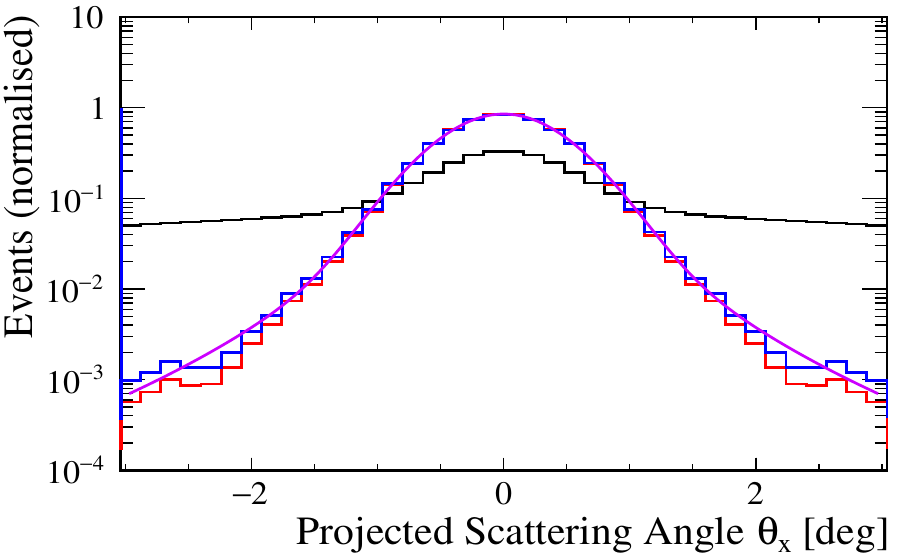
\includegraphics[width=0.8\textwidth]{Figures/muEDM_Dec2021/distributions.png}
            \caption{The angular distributions show: the full distribution (black), the distribution after cuts in the distance at the sample's plane (red), the distribution after acceptance correction (blue), and the fitted function for telescope characterization (violet).}
            \label{fig:muEDM:beamtime2021:distributions}
        \end{figure}
        
        \paragraph{Acceptance}
        The correction for the geometrical acceptance of the telescope was essential to accurately determine the tails of the angular distribution.
        To estimate the acceptance, for each upstream track identified, scattering angles were randomly assigned and added to a histogram, distinguishing instances within the acceptance of the most downstream sensor. 
        The ratio of histograms yielded the average acceptance as a function of projected scattering angles. 
        The acceptance correction was applied on a per-event basis, adjusting the scattering angles based on the acceptance value. 
        An example of such correction is shown in blue in Fig.~\ref{fig:muEDM:beamtime2021:distributions}
        
        \paragraph{Deconvolution}
        The method of track selection and acceptance correction was applied to both runs with and without the sample. 
        The distributions from these runs were then fitted.
        The process involved:
        \begin{outline}
            \1 Characterizing the telescope's response without the sample using a weighted sum of a Gaussian distribution and a Student's t distribution
            \1 Convolving the response function with the sample's angular distribution, assumed to follow a single Student's t distribution
            \1 using the negative log-likelihood to determine the best-fit parameters for describing the measured distribution with the sample
        \end{outline}
    
    \status{started}
    \subsection{Model evaluation and conclusions}
        This first beamtime aimed at testing the agreement between the Highland formula and the \gf Urb\'{a}n model for the multiple scattering in thin materials.
        The analysis of the data collected is still not finalized, but a rough agreement between data and models can be seen in Fig.~\ref{fig:muEDM:beamtime2021:results}.
        There are improvements that could be added to the analysis and/or to the simulation of the experimental setup, so updated results are expected in the following months.
        
    \begin{figure}   
            \centering
            \subfloat[Pokalon (orange), \SI{17}{\micro m} Graphite (blue), \SI{50}{\micro m} Graphite (violet), Silicon (red); circular markers for data at \SI{70}{MeV} and squared at \SI{90}{MeV}; error bars are the statistical uncertainties and the shaded area is the total uncertainties.]{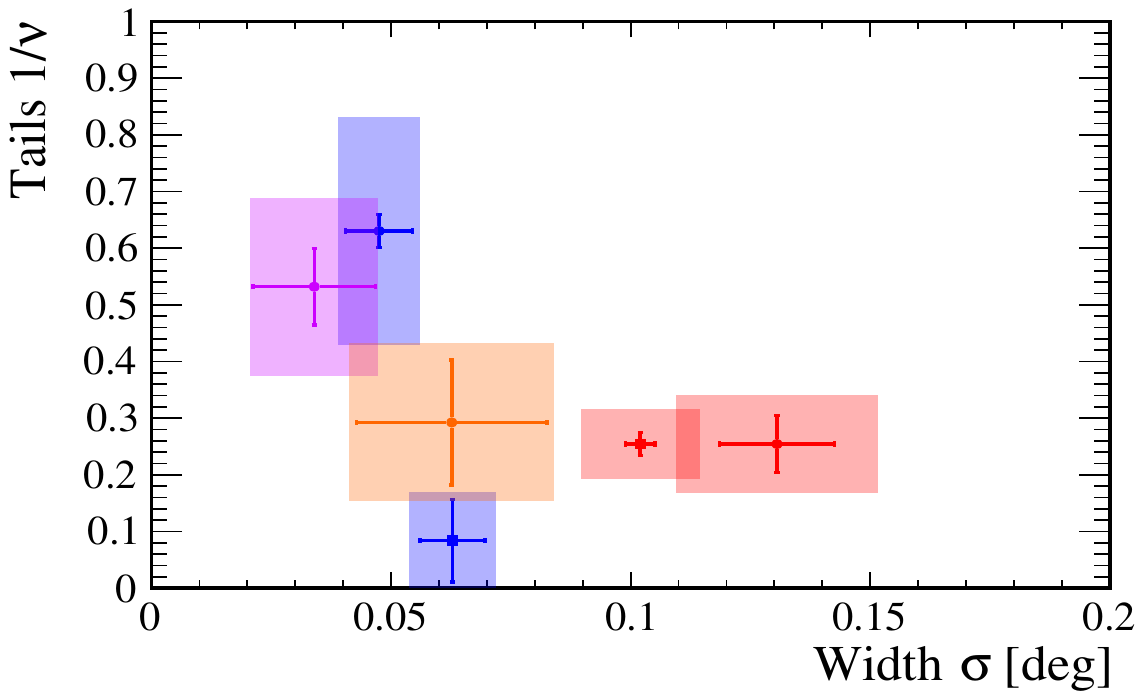
\includegraphics[width=0.48\textwidth, keepaspectratio]{Figures/muEDM_Dec2021/ms_fits.png}\label{fig:muEDM:beamtime2021:results:analysis}}
            \hfill
            \subfloat[Same color/shape coding as Fig.~\ref{fig:muEDM:beamtime2021:results:analysis} and the predictions of the Highland formula are shown by lines of width representing the uncertainty in thickness.]{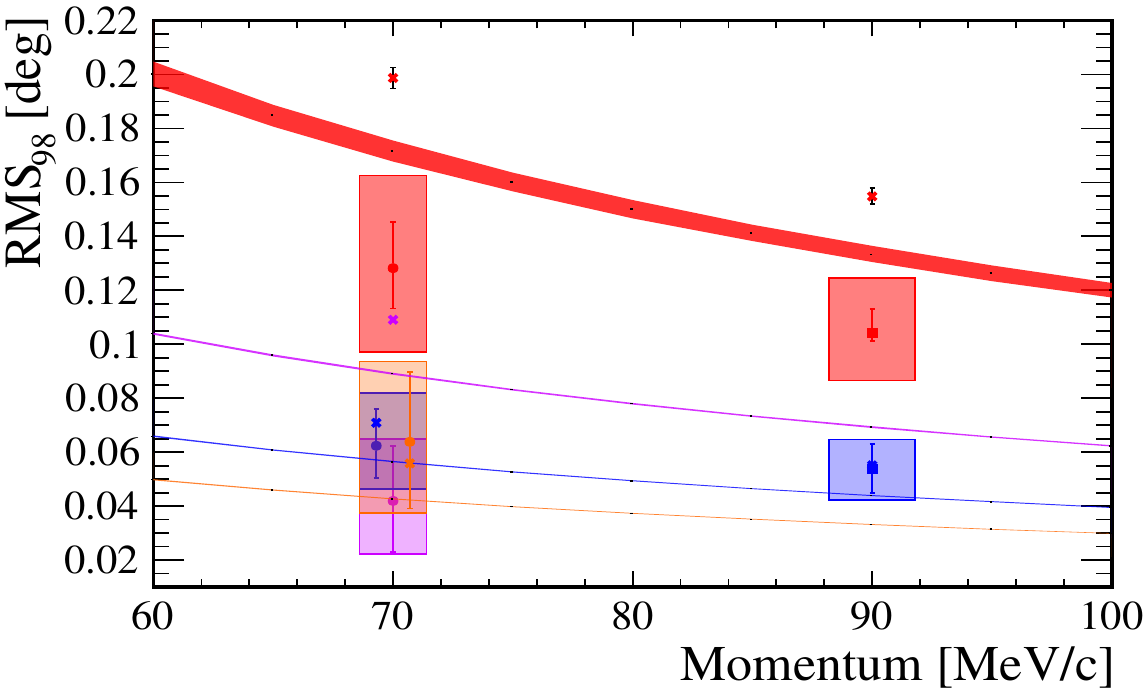
\includegraphics[width=0.48\textwidth, keepaspectratio]{Figures/muEDM_Dec2021/gf-highland_evaluation.png}\label{fig:muEDM:beamtime2021:results:models}}
            \caption{Results of the analysis of the different samples and confronted with predictions using the Highland formula and \gf. The details are not easy to read but the 'bring-home' message is that the results are somewhat in agreement and some improvement are planned on the analysis.}
            \label{fig:muEDM:beamtime2021:results}
        \end{figure}
        
\section{Beamtime 2022: Telescope and entrance detector}
    This second beamtime\footnote{Not counting the one for the \tpc + \grid of Sec.~\ref{sec:muEDM:gridpix:beamtime}, this is the second beamtime related to the entrance detector.} happened in November 2022.
    The amis where:
    \begin{outline}
        \1 Test of entrance scintillator with the additional `telescope'
        \1 parassitic measurements for the \tpc+ \grid
    \end{outline}
    This time I, togheter with Prof. Angela Papa and a David St\"{a}ger (a master student from ETH) partecipated actively in the development of the setup. 
    In particular we took care of the entrance scintillator, auxiliary detectors, the electronic, vacuum system, and one version of the telescope. 
    To test different reading options a second  telescope was developed by the Shanghai part of the collaboration and they also helped developing the mechanical structure.
    
    \subsection{Construction}
        \paragraph{Electronics}
        \paragraph{Scintillators}
        \paragraph{Final setup}
        \paragraph{Shanghai's version} 
    \begin{figure}   
            \centering
            \subfloat[Custom feed-throughs: PCB board, with soldered connectors, sealed with Stycast in a blind flange.]{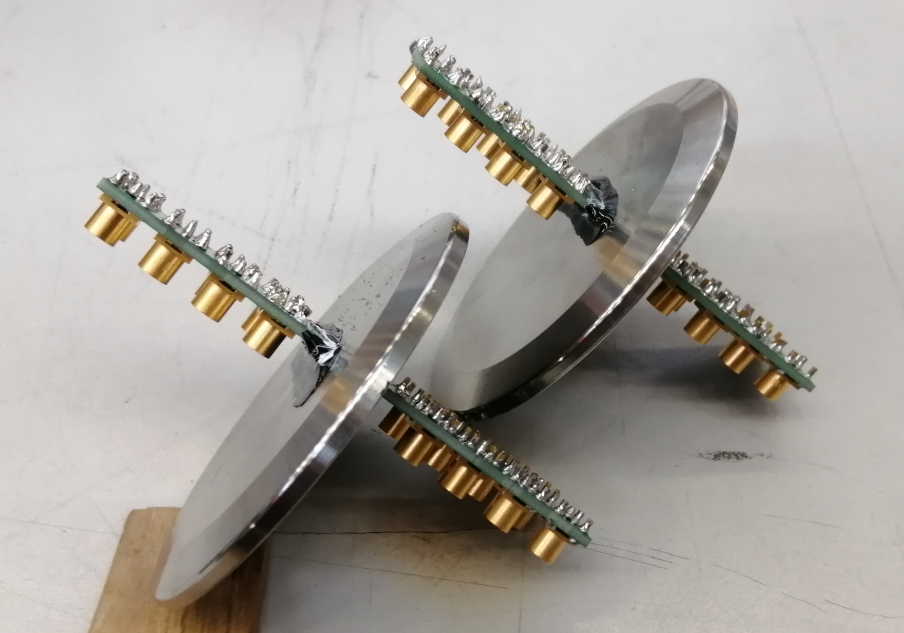
\includegraphics[width=0.49\textwidth, keepaspectratio]{Figures/muEDM_Nov2022/feedthrough.png}\label{}}
            \hfill
            \subfloat[A small PCB board with 3 SiPMs and one connector attached with optical cement to one of the scintillators.]{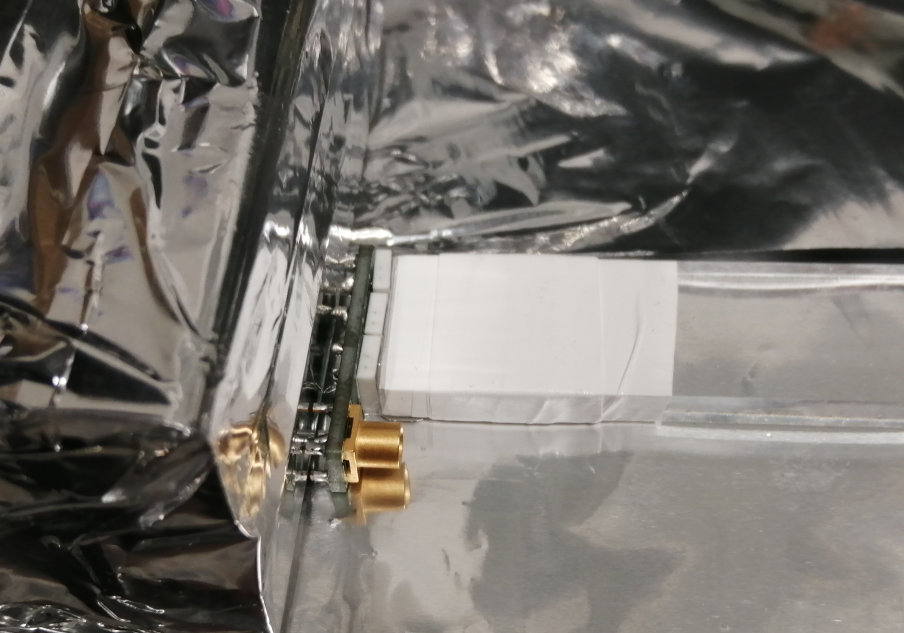
\includegraphics[width=0.49\textwidth, keepaspectratio]{Figures/muEDM_Nov2022/SIPMgluing.png}\label{}}
            \caption{Part of the preparation needed for the beamtime was to develop the detectors, as well as the vacuum in which the measurement would have taken place.}
            \label{fig:muEDM:beamtime2021:setup}
        \end{figure}
        
        \begin{figure}   
            \centering
            \subfloat[Assembly of the \textit{telescope} with \textit{entrance} and \textit{veto}.]{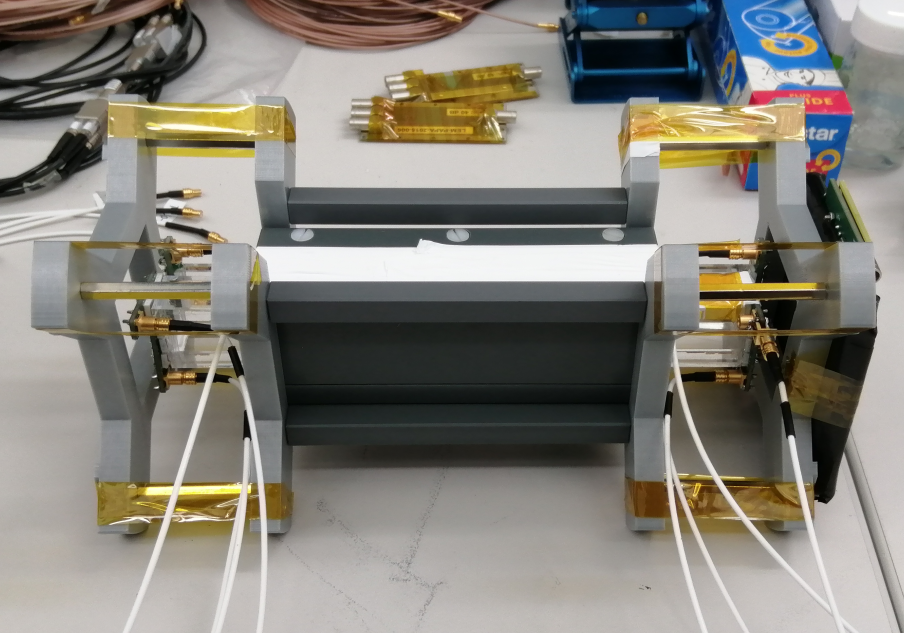
\includegraphics[width=0.49\textwidth, keepaspectratio]{Figures/muEDM_Nov2022/telescope_side.png}\label{}}
            \hfill
            \subfloat[``T'' beamline piece used as vacuum chamber.]{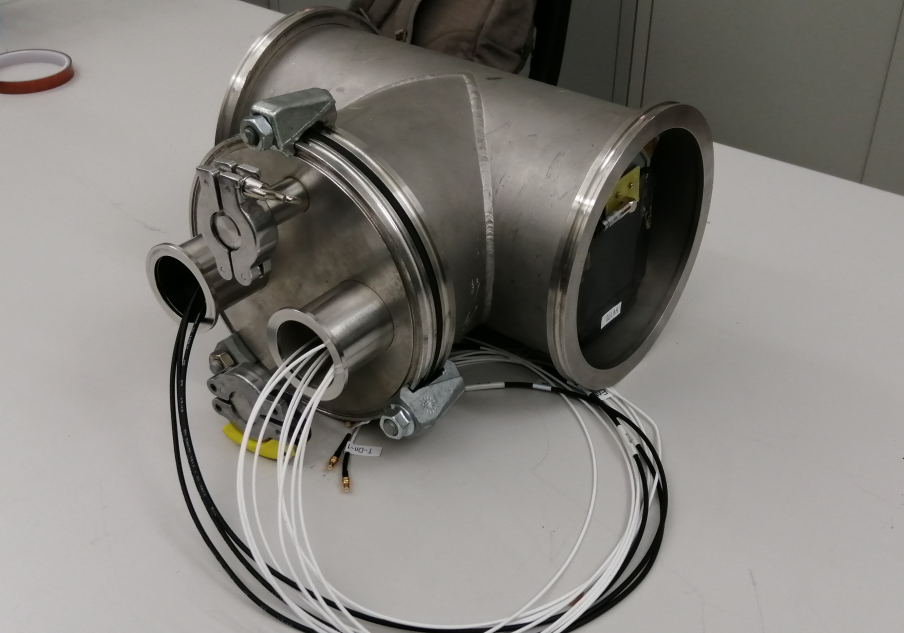
\includegraphics[width=0.49\textwidth, keepaspectratio]{Figures/muEDM_Nov2022/telescope_built.png}\label{}}
            \caption{The \textit{entrance} scintillator, the \textit{telescope}, and the \textit{veto} were assembled in a rigid structure. A ``T'' beamline piece was used to put the detector in the beamline. The lateral flange was adapted for the feedthroughs while, on the back, a \mylar widow was mounted to allow further measurements of the beam.}
            \label{fig:muEDM:beamtime2021:setup}
        \end{figure}
    \subsection{Data taking}
    \subsection{Data analysis}
    
\section{Beamtime 2023: Multi readout entrance}
\label{muEDM:beamtime2023}
    \subsection{Data taking}
    \subsection{Data analysis}

\status{started}
\printbibliography[
    heading = bibliographychapter,
    title=Bibliography on muEDM entrance detector
]

\end{refsection}


